\documentclass[11pt]{article}
\usepackage[T1]{fontenc}	%special characters
\usepackage[utf8]{inputenc}	%special characters

\usepackage{hyperref}
\usepackage[margin=1in]{geometry} %article layout margins
\usepackage{tabularx}		%tabulars width fixed textwidth
\usepackage{multicol}	%2 coloumns in Skills
\usepackage{graphicx}
\usepackage{sectsty}
\sectionfont{
	\sectionrule{0pt}{0pt}{-5pt}{0.8pt}
}

\begin{document}

\Large
\noindent
\textbf{Dirk Hornung, Ph.D.} \\

\normalsize
\noindent
\begin{minipage}{0.5\linewidth}
  \begin{tabularx}{0.6\textwidth}{>{\bfseries}l l}
    City:           & Barcelona \\
    Date of birth:  & 5th of October, 1991\\
    Place of birth: & Fulda, Germany \\
    Mobile:         & +34 695460404 \\
    E-mail:         & dirkhornung91@gmail.com \\
    Website:      	& www.dirkhornung.com
  \end{tabularx}
\end{minipage}
\begin{minipage}{0.5\linewidth}
  \begin{flushright}
    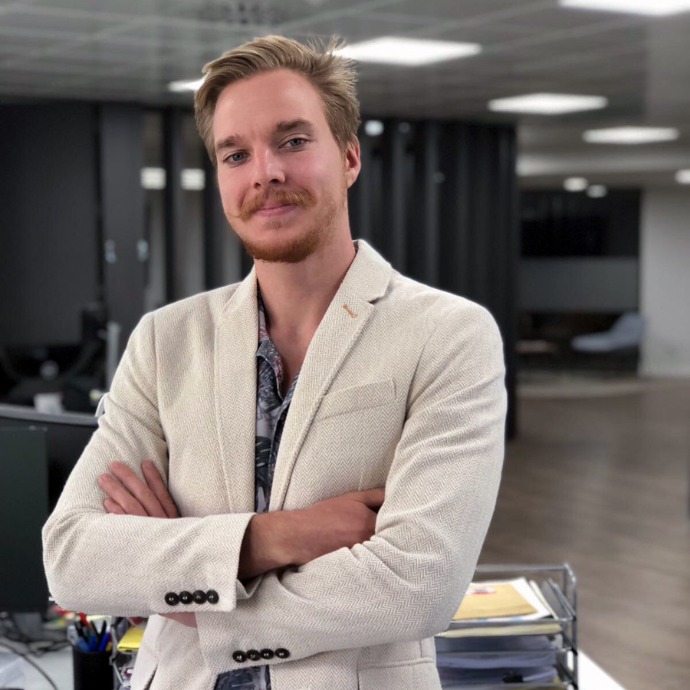
\includegraphics[width=0.4\textwidth]{dirk.png}
  \end{flushright}
\end{minipage}

% Cover Letter
% ------------------------------------------------------------------------------
% \section*{}
% \vspace{1cm}
% Dear Imagine, \\

% \noindent I am Dirk Hornung, a professional Ph.D. student at the institute of
% high energy physics of the "Universitat Autonoma de Barcelona". Right now I am
% researching Low-energy QCD and the determination of Standard Model Parameters.
% In principle I am finding intelligent ways to extract parameters of theoretical
% models out of experimental data. Apart from my studies I am working as a
% Blockchain and Full-Stack developer. \\

% \noindent My physical background demands a high level of skills in mathematics
% and analytical thinking. Within the past five years I obtained the skills to
% structure and solve problems of any kinds.  For visualizing and solving physic
% related problems I am using tools as Mathematica, Matlab, C++, Fortran and
% Python (Panda, NumPy, Matplotlib). Naturally as a physicist I have a broad
% spectrum of interests and always try to stay ahead of time. I am an experienced
% Decentralized Application (DApp) using Ethereum and
% IPFS on a daily basis. Furthermore I am a Full-Stack developer with a focus on
% React and Amazon Web Services (S3, Cognito, DynamoDB, RDS, Lambda). In my
% current projects I try to apply Machine Learning tools like Support Vector
% Machines and Convolutional Neural Networks using tensorflow. \\

% \noindent I am very confident that I would be an excellent choice for the Imagine
% Express 2019!\\

% \noindent Sincerely, \\
% Dirk Hornung \\

% \noindent P.S.
% Concerning Paris, je parle français!
% \newpage 
% ------------------------------------------------------------------------------

	
% \section*{Professional Profile}
% Theoretical solid-state and high-energy physicist. \\[1mm]
% Blockchain Developper \\[1mm]
% React Front End Developper \\[1mm]
% AWS Backend Developper \\[1mm]
% Data Analyst

\section*{Professional Experience}
\begin{tabularx}{\textwidth}{lX}
  2004 - present          & \textbf{Serious Entrepreneur} \\
                          & Hornung Webdesign, Eevents, Fulda Strategy Group
                            Gbr, FuldaCity, WeGoLoco, 17 \\\\
  Mai 2019 - January 2019 & \textbf{CYSAE} \\
                          & \textit{CTO} \\[1mm]
                          & Utility Token for Cuatre Casas, Certifying documents with the help of
                            Ethereum, Enterprise Democracy on Chain\\\\
                          % & https://www.cysae.com/  \\\\
  October 2017 - April 2019 & \textbf{Alda} \\
                            & \textit{CTO \& Co-Founder} \\[1mm]
                            & Fintech Chatbot helping Millenials in Financial Education\\\\
                            % & https://www.alda.bot/
  % 2017 & \textbf{WeGoLoco} \\
  %              & \textit{CTO \& Co-Founder} \\[1mm]
  %              & Matchin Tinder with the Local Commerce \\[1mm]

  % 2017 & \textbf{FuldaCity} \\
  %              & \textit{CTO \& Co-Founder} \\[1mm]
  %              & Bringing my Hometown online within the Meteor/React Framework \\[1mm]
  %              & http://www.fuldacity.de/  \\\\
  
  %              % \pagebreak
  
  % 2016 & \textbf{Emexs} \\
  %              & \textit{Backend Developper/ Data Analyst} \\[1mm]
  %              & Finding smart algorithms to forecast future prices in the hotel sector \\[1mm]
  %              & http://www.elprat.cat/ (Drupal) \\\\
  %              & http://www.hotelsdot.com/ (Codeigniter) \\\\
  
  
  % 2013 - 2016 & \textbf{Fulda Strategy Group GbR - Management Consultancy} \\
  %              & \textit{Founder and Managing Director} \\[1mm]
  %              & Projects in the area of ERP selection and implementation, process management and software development \\[1mm]
  %              & www.fulda-strategy.com \\\\
  
  % 2010 - present & \textbf{Eevents Fulda Gbr - Event Management} \\
  %              & \textit{Founder} \\[1mm]
  %              & Organising of company events, weddings and birthdays \\[1mm]
  %              & www.eevents-fulda.de \\\\
  
  % 2010 - 2014 & \textbf{Hornung Webdesign - Webdesign Agency} \\
  %              & \textit{Founder} \\[1mm]
  %              & Developing and maintaining of CMS and SaaS. \\\\
\end{tabularx}


\section*{Education}
\begin{tabularx}{\textwidth}{sX}
  2015 - 2019  & Ph.D., Theoretical Physics, Autonomous University of
                 Barcelona (Spain) \\
               & Thesis: The QCD Strong Coupling from Hadronic Tau
                 Decays \\
               & Supervisor: Dr. Matthias Jamin \\\\
  2014 - 2015  & M.Sc., Particle Physics,Autonomous University of
                                Barcelona (Spain) \\
               & Thesis: 1-Loop Anomalous Dimensions of 4-Quark
                 Operators \\
               & Supervisor: Dr. Matthias Jamin \\\\
  2011 - 2014  & B.Sc., Condensed Matter Physics, Goethe University Frankfurt (Germany) \\
               & Thesis: Band Structure Studies of Graphene and Modified
                 Graphene Structure \\
               & Supervisor: Prof. Dr. Roser Valentí
\end{tabularx}
		

\section*{Skills}
\begin{tabularx}{\textwidth}{sX}
  Hard Skills  & Ph.D., Theoretical Physics, Autonomous University of
                 Barcelona (Spain) \\
               & Thesis: The QCD Strong Coupling from Hadronic Tau
                 Decays \\
               & Supervisor: Dr. Matthias Jamin \\\\
  2014 - 2015  & M.Sc., Particle Physics,Autonomous University of
                 Barcelona (Spain) \\
               & Thesis: 1-Loop Anomalous Dimensions of 4-Quark
                 Operators \\
               & Supervisor: Dr. Matthias Jamin \\\\
  2011 - 2014  & B.Sc., Condensed Matter Physics, Goethe University Frankfurt (Germany) \\
               & Thesis: Band Structure Studies of Graphene and Modified
                 Graphene Structure \\
               & Supervisor: Prof. Dr. Roser Valentí
\end{tabularx}
\begin{multicols}{2}
  \begin{itemize}
    \renewcommand\labelitemi{-}
  \item Javascript, Swift, PHP, SQL, CSS, HTML 
  \item React, React Native, Meteor, Laravel
  \item Wordpress, Goole Analytics, SEO
  \item Data \& Statistics Analysis
  \item AWS (DynamoDB, S3, Cognito, Lambda)
    \columnbreak
  \item Fortran, C++, Solidity
  \item Matlab, Mathematica
  \item Photoshop, Illustrator, After Effects
  \item Unix Shell, Linux
  \end{itemize}
\end{multicols}
		


	% \section*{Funding}
	% \begin{tabularx}{\textwidth}{sX}
	% 	2015 - present & Ph.D. PIF grant at the Autònoma de Barcelona (Spain), 1200 \euro / month 
	% \end{tabularx}


	% \section*{Teaching Experience}
	% 	\begin{tabularx}{\textwidth}{sX}
	% 		2015 - 2018 & Universitat Autònoma de Barcelona, Theoretical Mechanics/
  %                   Quantum Mechanics I/ Quantum Mechanics II, Complex Numbers/
  %                   Teaching Assistant (spanish) \\[1mm]
	% 		\centering{2014} & Goethe Universität Frankfurt, Quantum Mechanics I , exercise tutor \\
	% 		& Goethe Universität Frankfurt, Math for Physicists II, exercise tutor \\[1mm]
	% 		2013 - 2014 & Goethe Universität Frankfurt, Math for Physicists I, exercise tutor
	% 	\end{tabularx}


	% \section*{Publications}
	% 	\begin{tabularx}{\textwidth}{sX}
	% 		2015 & Diogo Boito, \textbf{Dirk Hornung}, Matthias Jamin \\[1mm]
	% 		& "Anomalous dimensions of four-quark operators and renormalon structure of mesonic two-point correlators" \\[2mm]
	% 		&  \textit{arXiv:1510.03812 [hep-ph]}	
	% 	\end{tabularx}


	% \section*{Oral presentations}
	% 	\begin{tabularx}{\textwidth}{sX}
  %     2018 & Aix Marseille Université, ``Determination of the QCD Coupling from
  %            ALEPH $\tau$-Decay data''
	% 	\end{tabularx}\vspace{1mm}
	% 	\begin{tabularx}{\textwidth}{sX}
	% 	2015 & Universitat Autònoma de Barcelona, Master Thesis Defense of : \\ & ``1-Loop anomalous dimensions of 4-quark operators''
	% 	\end{tabularx}\vspace{1mm}
	% 	\begin{tabularx}{\textwidth}{sX}
	% 		2014 & Goethe Universität Frankfurt, Group Seminar Talk: ``Band structure studies of graphene and modified graphene structures''
	% 	\end{tabularx}

	\section*{Languages}
	\begin{tabularx}{\textwidth}{sX}
		German: & native \\
		English: & proficient \\
		Spanish: & proficient \\
		French: & intermediate \\
		Hungarian: & basics 
	\end{tabularx}
	

%	\section*{References}
%	\begin{tabularx}{0.5\textwidth}{@{}l}
%		Prof. Dr. Roser Valentí \\
%		valenti@itp.uni-frankfurt.de \\
%		+49 69 798 47816 \\
%		Institut für Theoretische Physik \\
% 		Goethe-Universität Frankfurt am Main \\
% 		Max-von-Laue-Strasse 1 \\
%		60438 Frankfurt am Main \\
%		Germany 	
%	\end{tabularx}
%	\begin{tabularx}{0.5\textwidth}{ll}
%		Prof. Dr. Matthias Jamin \\
%		jamin@ifae.es \\
%		Institut de Fisica d'Altes Energies (IFAE) \\
%                Universitat Autònoma de Barcelona \\
%                Plaça Cívica \\
%                08193 Cerdanyola \\
%		Spain \\
%		\\
%	\end{tabularx}
	

\end{document}
